\section{ตัวแบบเชิงแปรผันสำหรับต่อเติมภาพเฉดเทา}\label{inpaint-model-grayscale}

\hspace{1cm} กำหนดให้ $ u: \Omega \rightarrow V,\ z: \Omega \rightarrow V$ แทนภาพที่ได้รับการต่อเติมและภาพที่ต้องการต่อเติม ตามลำดับ

\begin{figure}[H]
	\centering
	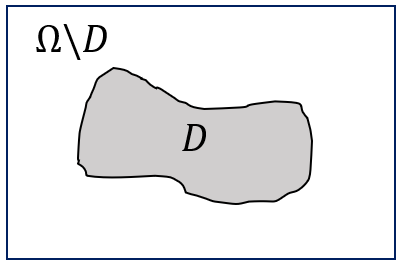
\includegraphics[width=0.375\linewidth]{image/sample-domain.png}
	\caption{$D$ แทนโดเมนต่อเติม}
	\label{figure:sample-domain}
\end{figure}

\hspace{1cm} การต่อเติมภาพเฉดเทาคือการหาค่าเหมาะสมที่สุดของค่าความเข้มของภาพในบริเวณโดเมนต่อเติม $D$ โดยใช้ข้อมูลที่มีอยู่ใน $\Omega \textbackslash D$ 

\hspace{1cm} Chan และ Shen \cite{ref:rof-inpaint-chan-shen} ได้นำเสนอตัวแบบเชิงการแปรผัน (variational model) ที่ใช้เร็กกิวลาร์ไรซ์เซชันแบบการแปรผันรวม (Total variation based regularization) โดยพัฒนาต่อจากตัวแบบ ROF สำหรับการกำจัดสัญญาณรบกวน \cite{ref:ROF-template} ซึ่งตัวแบบเชิงการแปรผันนี้กำหนดโดย
\begin{align}
    \min_{u} \{ \mathcal{J}(u) = \frac{1}{2} \int_{\Omega}\lambda (u-z)^2 d\Omega +  \int_{\Omega}  |\nabla u|  d\Omega \}
\label{e1}
\end{align}

เมื่อ 
\begin{align}
    \lambda=\lambda(\mathbf{x}) = \left \{ \begin{array}{ll}  \lambda_0, & x \in \Omega \setminus D \\ 0, & x \in D  \end{array} \right . 
    \label{e2}
\end{align}
แทนพารามิเตอร์เร็กกิวลาร์ไรซ์เซชัน (regularization parameter) และ $\lambda_0 >0$
